% Projeto de Pesquisa -- UEMA/Uemanet -- compilar com pdfLaTeX (padrão do Overleaf)
\documentclass[12pt,a4paper]{article}
\usepackage[utf8]{inputenc}
\usepackage[T1]{fontenc}
\usepackage[brazil]{babel}
\usepackage[scaled=1]{helvet}      % Helvetica/Nimbus Sans: métrica equivalente à do Arial
\renewcommand{\familydefault}{\sfdefault}
\usepackage[a4paper,top=3cm,left=3cm,bottom=2cm,right=2cm,headsep=1cm]{geometry}
\usepackage{setspace}
\usepackage{titlesec}
\usepackage{tocloft}
\usepackage{fancyhdr}
\usepackage{graphicx}
\usepackage{array}
\usepackage[table]{xcolor}
\usepackage{url}
\urlstyle{same}
\usepackage[hyphens]{url}
\Urlmuskip=0mu plus 1mu
\sloppy
\onehalfspacing
\setlength{\parindent}{1.25cm}
\setlength{\parskip}{0pt}
\raggedbottom

% Títulos (NBR 6024): primária em maiúsculas/negrito; secundária negrito; terciária negrito itálico
\titleformat{\section}{\normalfont\normalsize\bfseries}{\thesection}{1ex}{}
\titleformat{\subsection}{\normalfont\normalsize\bfseries}{\thesubsection}{1ex}{}
\titleformat{\subsubsection}{\normalfont\normalsize\bfseries\itshape}{\thesubsubsection}{1ex}{}
\titlespacing*{\section}{0pt}{0pt}{18pt}
\titlespacing*{\subsection}{0pt}{18pt}{18pt}
\titlespacing*{\subsubsection}{0pt}{18pt}{18pt}

% Sumário
\addto\captionsbrazil{\renewcommand{\contentsname}{SUMÁRIO}}
\renewcommand{\cfttoctitlefont}{\hfill\normalfont\normalsize\bfseries}
\renewcommand{\cftaftertoctitle}{\hfill\mbox{}}
\renewcommand{\cftsecfont}{\bfseries}
\renewcommand{\cftsecpagefont}{\bfseries}
\renewcommand{\cftsecleader}{\bfseries\cftdotfill{\cftdotsep}}
\setlength{\cftbeforesecskip}{4pt}
\setlength{\cftbeforesubsecskip}{2pt}
\setlength{\cftsecindent}{0pt}\setlength{\cftsecnumwidth}{1.3cm}
\setlength{\cftsubsecindent}{0pt}\setlength{\cftsubsecnumwidth}{1.3cm}
\setlength{\cftsubsubsecindent}{0pt}\setlength{\cftsubsubsecnumwidth}{1.8cm}

% Número de página: 10 pt, canto superior direito
\pagestyle{empty}
\fancypagestyle{texto}{\fancyhf{}\fancyhead[R]{\fontsize{10}{12}\selectfont\thepage}\renewcommand{\headrulewidth}{0pt}}

\begin{document}

% ---------- CAPA (não contada) ----------
\begin{titlepage}
\centering\singlespacing
\textbf{UNIVERSIDADE ESTADUAL DO MARANHÃO}\\
\textbf{NÚCLEO DE TECNOLOGIAS PARA EDUCAÇÃO}\\
\textbf{CURSO SUPERIOR DE TECNOLOGIA EM ANÁLISE E DESENVOLVIMENTO DE SISTEMAS}\par
\vspace{3.2cm}
\textbf{PAULO RICARDO COIMBRA SOUSA}\par
\vspace{3.2cm}
\textbf{FILTRAGEM DNS COM PI-HOLE EM SERVIDOR LOCAL:} proposta de controle de acesso a conteúdos indevidos na rede de um prédio público municipal\par
\vfill
\textbf{Grajaú – MA}\\
\textbf{2026}
\end{titlepage}
\setcounter{page}{1}

% ---------- FOLHA DE ROSTO ----------
\begin{titlepage}
\centering\singlespacing
\textbf{PAULO RICARDO COIMBRA SOUSA}\par
\vspace{3.6cm}
\textbf{FILTRAGEM DNS COM PI-HOLE EM SERVIDOR LOCAL:} proposta de controle de acesso a conteúdos indevidos na rede de um prédio público municipal\par
\vspace{1.2cm}
\hfill\begin{minipage}{8cm}\raggedright\singlespacing
Projeto de pesquisa apresentado ao curso Superior de Tecnologia em Análise e Desenvolvimento de Sistemas como requisito da disciplina de TCC, para fins de planejamento, organização e elaboração de trabalhos científicos.\par\vspace{12pt}
Orientador: Prof. Me. Paulo Ericson Valentim Silva.
\end{minipage}
\vfill
\textbf{Grajaú – MA}\\
\textbf{2026}
\end{titlepage}

% ---------- SUMÁRIO ----------
\clearpage
\singlespacing\tableofcontents\onehalfspacing

\clearpage\pagestyle{texto}
\section{INTRODUÇÃO}
A informatização dos serviços públicos municipais avançou de forma expressiva na última década. Segundo a pesquisa TIC Governo Eletrônico 2023, que ouviu 4.265 prefeituras, 91\% delas já disponibilizavam ao menos um serviço digital ao cidadão, contra 75\% dez anos antes (CENTRO REGIONAL DE ESTUDOS PARA O DESENVOLVIMENTO DA SOCIEDADE DA INFORMAÇÃO, 2024). Essa expansão, porém, não foi acompanhada na mesma proporção pela estruturação da segurança da informação: a mesma pesquisa aponta que apenas 33\% das prefeituras contavam com centro de operações para monitoramento de tráfego, segurança e emergências, índice que chega a 84\% somente nos municípios com mais de 500 mil habitantes (CENTRO REGIONAL DE ESTUDOS PARA O DESENVOLVIMENTO DA SOCIEDADE DA INFORMAÇÃO, 2024). Em outras palavras, a maior parte dos municípios brasileiros, especialmente os de pequeno e médio porte, como grande parte dos maranhenses, opera redes conectadas à internet com pouca ou nenhuma camada de proteção e de controle.

Os efeitos dessa fragilidade já são visíveis. Em 2025, ataques cibernéticos interromperam serviços de prefeituras como as de São José do Rio Preto (SP), Paranhos (MS) e Porto Nacional (TO), afetando emissão de notas fiscais, agendamento de consultas e sistemas de arrecadação; dados do Centro de Prevenção, Tratamento e Resposta a Incidentes Cibernéticos de Governo indicam que, em apenas sete meses de 2025, os incidentes contra sistemas governamentais superaram os totais anuais de 2021, 2022 e 2023 (ARRUDA, 2025). Grande parte desses ataques começa com uma ação simples do usuário final, como o acesso a uma página maliciosa, o clique em um \textit{link} de \textit{phishing} ou o \textit{download} de um arquivo infectado, o que coloca a navegação na \textit{web} no centro do problema.

Paralelamente ao risco técnico, existe um problema de conduta e de responsabilidade. A rede de um prédio público é um bem público, e seu uso para acessar conteúdo sexual, sítios de apostas ou, em casos extremos, material de natureza criminosa, como o que envolve abuso sexual de crianças e adolescentes, tipificado pelo Estatuto da Criança e do Adolescente (BRASIL, 1990), expõe a administração a danos de imagem, a responsabilização e ao desperdício de recursos. A norma ABNT NBR ISO/IEC 27002 inclui, entre seus controles, a filtragem da \textit{web} como meio de reduzir a exposição a conteúdo malicioso e de impedir o acesso a recursos externos não autorizados (ASSOCIAÇÃO BRASILEIRA DE NORMAS TÉCNICAS, 2022b), e o \textit{Center for Internet Security} recomenda o uso de serviços de filtragem DNS em todos os ativos da organização como salvaguarda básica (CENTER FOR INTERNET SECURITY, 2024).

Soluções comerciais de filtragem de conteúdo, como \textit{firewalls} de próxima geração e \textit{proxies} com inspeção de tráfego, existem, mas geralmente envolvem licenças anuais e exigem mão de obra especializada, o que as torna pouco acessíveis à realidade da maioria das prefeituras. Nesse cenário, o Pi-hole surge como alternativa: trata-se de um software livre que atua como servidor DNS (\textit{Domain Name System}) da rede local e que responde com um endereço nulo às consultas por domínios presentes em listas de bloqueio, impedindo que qualquer dispositivo da rede alcance esses destinos, sem necessidade de instalar programas nas estações de trabalho (PI-HOLE, 2025a). Embora seja popularmente associado ao Raspberry Pi, o Pi-hole pode ser instalado em qualquer servidor Linux, inclusive em um computador reaproveitado ou em uma máquina virtual, solução adotada neste projeto por oferecer maior capacidade de processamento, armazenamento e estabilidade para um ambiente institucional.

Diante desse contexto, este projeto delimita-se ao estudo da implantação do Pi-hole em servidor local, como filtro DNS, na rede de \textbf{um} prédio público municipal de Sítio Novo/MA, com foco no bloqueio de quatro categorias de conteúdo: (i) sexual/pornográfico; (ii) apostas \textit{on-line}; (iii) domínios maliciosos (\textit{malware} e \textit{phishing}); e (iv) domínios associados a conteúdo de natureza criminosa presentes em listas públicas. Ficam fora do escopo a inspeção do conteúdo de tráfego cifrado (HTTPS), a autenticação individual de usuários, o controle de dispositivos que utilizem redes móveis próprias (4G/5G) e a filtragem de conteúdos específicos dentro de sítios permitidos, limites que serão discutidos ao longo do trabalho.

Este projeto está organizado em cinco seções. Após esta introdução, a seção 2 apresenta os objetivos geral e específicos. A seção 3 traz o referencial teórico, abordando a segurança da informação na administração pública, o funcionamento do DNS, a filtragem baseada em DNS, o Pi-hole e seus limites, além dos aspectos legais envolvidos. A seção 4 descreve a metodologia, incluindo a proposta tecnológica preliminar, e a seção 5 apresenta o cronograma de execução. Seguem-se as referências e os apêndices.

\subsection{Problema e questão norteadora}
Prédios públicos municipais, em geral, oferecem acesso à internet a servidores e, por vezes, a visitantes, sem qualquer mecanismo de filtragem, deixando a rede vulnerável a ameaças digitais e sem meios de coibir o acesso a conteúdo incompatível com o ambiente de trabalho e com a moralidade administrativa. Ao mesmo tempo, a escassez de orçamento e de pessoal técnico dificulta a adoção de soluções comerciais. Assim, a pesquisa será guiada pela seguinte questão norteadora: \textbf{em que medida a implantação do Pi-hole em um servidor local, como filtro DNS, é capaz de controlar o acesso de servidores públicos a sítios indevidos e maliciosos na rede de um prédio público municipal, com baixo custo e sem prejudicar o desempenho da navegação?}

\subsection{Justificativa}
A relevância social do estudo reside na proteção do patrimônio informacional público e na promoção do uso adequado de um recurso custeado pelo contribuinte. Ao bloquear domínios maliciosos antes mesmo que a conexão seja estabelecida, a filtragem DNS reduz a superfície de ataque da rede e atua como uma camada preventiva contra \textit{ransomware} e \textit{phishing}, ameaças que, como visto, já paralisaram serviços de prefeituras brasileiras (ARRUDA, 2025). Ao bloquear categorias de conteúdo impróprio, contribui para que a administração cumpra os princípios constitucionais da moralidade e da eficiência e para que disponha de evidências técnicas, ainda que agregadas, em casos de uso indevido.

A relevância institucional decorre do alinhamento com as políticas públicas de segurança da informação. A Política Nacional de Segurança da Informação (BRASIL, 2018a) e a Política Nacional de Cibersegurança (BRASIL, 2023) estabelecem diretrizes para a proteção dos ativos de informação na administração pública, e o Programa de Privacidade e Segurança da Informação (PPSI), da Secretaria de Governo Digital, organiza seus controles com base no CIS Controls, incluindo o controle dedicado às proteções de \textit{e-mail} e de navegador \textit{web} (BRASIL, 2024). Embora tais normas sejam voltadas prioritariamente à esfera federal, servem de referência para estados e municípios, que carecem de modelos práticos e acessíveis para aplicá-las.

A relevância acadêmica está em produzir um estudo aplicado, com avaliação mensurável, sobre uma ferramenta amplamente utilizada em ambientes domésticos, mas ainda pouco investigada em contextos institucionais públicos. A literatura recente começa a explorar o Pi-hole em ambientes educacionais (ELAVARASI \textit{et al.}, 2026), porém não foram localizados, no levantamento preliminar, estudos voltados especificamente à administração pública municipal brasileira, com suas particularidades legais, como a necessidade de conciliar o controle de acesso com a Lei Geral de Proteção de Dados Pessoais (BRASIL, 2018b).

Por fim, a escolha do tema relaciona-se com a formação no curso de Tecnologia em Análise e Desenvolvimento de Sistemas, especialmente com os conteúdos de redes de computadores, sistemas operacionais e segurança da informação, e com a necessidade observada de evitar o uso indevido das redes públicas de internet, o que motivou a busca por uma solução acessível de controle de acesso.

\subsection{Hipóteses}
A pesquisa será norteada pelas hipóteses abaixo, que, no percurso da investigação, serão confirmadas ou refutadas:

{\leftskip=1.25cm\noindent\hangindent=0.6cm a)~ o Pi-hole, instalado em servidor local e configurado com listas de bloqueio por categoria, bloqueia a maior parte dos domínios de teste das categorias definidas, com baixa incidência de bloqueios indevidos de serviços legítimos e sem aumento perceptível no tempo de resposta das consultas DNS;\par}
{\leftskip=1.25cm\noindent\hangindent=0.6cm b)~ o recurso de gerenciamento de grupos do Pi-hole permite aplicar políticas de filtragem diferenciadas por setor ou segmento da rede, sem custo de licenciamento;\par}
{\leftskip=1.25cm\noindent\hangindent=0.6cm c)~ a eficácia do Pi-hole como ferramenta de controle depende de medidas complementares no roteador ou \textit{firewall}, como o bloqueio de servidores DNS externos e de serviços conhecidos de DNS cifrado, sem as quais o filtro pode ser facilmente contornado.\par}
\clearpage
\section{OBJETIVOS}
Os objetivos a seguir orientam o desenvolvimento da pesquisa.

\subsection{Objetivo Geral}
Avaliar a eficácia do Pi-hole, implantado em servidor local, como ferramenta de segurança e de controle de acesso a conteúdos indevidos na rede de um prédio público municipal de Sítio Novo/MA.

\subsection{Objetivos Específicos}
Para alcançar o objetivo geral, serão realizadas as seguintes ações:

{\leftskip=1.25cm\noindent\hangindent=0.6cm a)~ diagnosticar a infraestrutura de rede e as práticas de uso da internet no prédio público municipal selecionado;\par}
{\leftskip=1.25cm\noindent\hangindent=0.6cm b)~ implantar e configurar o Pi-hole em servidor local, com listas de bloqueio por categoria, grupos por setor e medidas complementares contra o contorno do filtro;\par}
{\leftskip=1.25cm\noindent\hangindent=0.6cm c)~ mensurar a eficácia do bloqueio, a ocorrência de falsos positivos e o impacto no desempenho das consultas DNS por meio de testes em ambiente controlado;\par}
{\leftskip=1.25cm\noindent\hangindent=0.6cm d)~ elaborar um modelo documentado de implantação e uma minuta de política de uso aceitável da internet, passíveis de replicação em outros prédios da administração municipal.\par}
\clearpage
\section{REFERENCIAL TEÓRICO}
Esta seção reúne os conceitos que sustentam a pesquisa, partindo do contexto mais amplo da segurança da informação na administração pública até chegar às características técnicas e aos limites do Pi-hole, objeto central do estudo.

\subsection{Segurança da informação na administração pública}
A segurança da informação é tradicionalmente definida pela preservação de três propriedades: confidencialidade, integridade e disponibilidade. Stallings e Brown (2014) destacam que essas propriedades não são garantidas por um único mecanismo, mas por um conjunto de controles sobrepostos, organizados em camadas, de modo que a falha de um deles seja compensada pelos demais. Essa noção de defesa em profundidade é fundamental para esta pesquisa, pois a filtragem DNS não pretende substituir antivírus, atualizações ou \textit{backups}, e sim acrescentar uma camada preventiva situada antes do estabelecimento da conexão.

No plano normativo, a ABNT NBR ISO/IEC 27001 estabelece os requisitos de um sistema de gestão da segurança da informação baseado em análise de riscos (ASSOCIAÇÃO BRASILEIRA DE NORMAS TÉCNICAS, 2022a), enquanto a ABNT NBR ISO/IEC 27002 detalha os controles aplicáveis, entre os quais se encontra a filtragem da \textit{web}, voltada a reduzir a exposição a conteúdo malicioso e a impedir o acesso a recursos externos não autorizados (ASSOCIAÇÃO BRASILEIRA DE NORMAS TÉCNICAS, 2022b). O \textit{Center for Internet Security} segue linha semelhante e, em seu conjunto de controles críticos, recomenda expressamente o uso de serviços de filtragem DNS para bloquear o acesso a domínios maliciosos conhecidos (CENTER FOR INTERNET SECURITY, 2024). A convergência entre essas referências indica que a filtragem de navegação é reconhecida como boa prática, e não como medida excepcional.

No Brasil, a Política Nacional de Segurança da Informação (BRASIL, 2018a) e a Política Nacional de Cibersegurança (BRASIL, 2023) definem princípios e objetivos para a proteção dos ativos de informação do Estado. Para operacionalizá-los, a Secretaria de Governo Digital criou o PPSI, cujo guia de \textit{framework} adota o CIS Controls como base e inclui um controle específico para proteções de \textit{e-mail} e navegador \textit{web} (BRASIL, 2024). Há, contudo, uma lacuna entre esse arcabouço, pensado para órgãos federais com equipes estruturadas, e a realidade municipal. Os dados da pesquisa TIC Governo Eletrônico, que revelam baixa presença de centros de monitoramento nas prefeituras menores (CENTRO REGIONAL DE ESTUDOS PARA O DESENVOLVIMENTO DA SOCIEDADE DA INFORMAÇÃO, 2024), e o aumento dos incidentes contra órgãos públicos (ARRUDA, 2025) reforçam a necessidade de soluções simples, de baixo custo e documentadas, que traduzam essas diretrizes para a escala de um prédio municipal. É nesse espaço que se insere a presente proposta.

\subsection{O sistema de nomes de domínio (DNS)}
Para compreender por que o DNS é um ponto estratégico de controle, é necessário entender seu papel. O DNS é o serviço que traduz nomes de domínio legíveis por humanos, como "www.exemplo.gov.br", em endereços IP utilizados pelos equipamentos de rede. Sua arquitetura foi especificada por Mockapetris (1987a, 1987b) como uma base de dados hierárquica e distribuída, na qual servidores raiz, servidores de domínio de topo e servidores autoritativos cooperam para responder às consultas. Kurose e Ross (2021) explicam que, na prática, o computador do usuário envia a consulta a um servidor DNS local, normalmente informado pelo protocolo DHCP, que realiza a resolução em nome do cliente e armazena as respostas em \textit{cache} para acelerar consultas futuras.

Essa característica é o que torna o DNS um ponto de controle privilegiado. Como praticamente toda comunicação na internet começa com uma consulta DNS, quem controla o servidor DNS local consegue decidir, antes de qualquer conexão, quais nomes serão resolvidos e quais não serão. Tanenbaum, Feamster e Wetherall (2021) observam que o DNS foi concebido sem mecanismos nativos de segurança, o que o expõe a ataques como envenenamento de \textit{cache} e redirecionamento malicioso; a mesma fragilidade, no entanto, é explorada de forma defensiva pela filtragem DNS. Khormali \textit{et al.} (2020), em revisão sobre segurança e privacidade do DNS, mostram que o protocolo é simultaneamente vetor de ataques, como tunelamento de dados e uso de domínios gerados algoritmicamente por \textit{malware}, e fonte valiosa de observação para defesa, justamente por concentrar a intenção de acesso de todos os dispositivos da rede.

\subsection{Filtragem baseada em DNS e \textit{DNS sinkhole}}
A filtragem DNS consiste em interceptar as consultas da rede e comparar o domínio solicitado com listas de bloqueio. Quando o domínio consta da lista, o servidor devolve uma resposta nula ou um endereço inválido, técnica chamada de \textit{DNS sinkhole}, e o dispositivo simplesmente não consegue estabelecer a conexão. A Agência de Segurança Nacional e a Agência de Segurança Cibernética e de Infraestrutura dos Estados Unidos denominam esse tipo de serviço de \textit{Protective DNS} e recomendam sua adoção por permitir bloquear, em um único ponto, o acesso a domínios de \textit{malware}, \textit{phishing} e comando e controle, além de produzir registros úteis para a detecção de incidentes (NATIONAL SECURITY AGENCY; CYBERSECURITY AND INFRASTRUCTURE SECURITY AGENCY, 2021). A revisão mais recente do guia de implantação segura de DNS do NIST também incorpora o \textit{Protective DNS} entre as práticas recomendadas para organizações (ROSE; LIU; GIBSON, 2026).

A eficácia desse modelo, porém, depende diretamente da qualidade das listas utilizadas. Kührer, Rossow e Holz (2014), ao avaliarem listas públicas de domínios maliciosos, constataram que elas apresentam coberturas muito distintas, que nenhuma lista isolada é suficiente e que a atualização frequente é decisiva, pois domínios maliciosos têm vida curta. Para a filtragem de categorias de conteúdo, como sítios adultos e de apostas, existem listas mantidas por comunidades e instituições, como o repositório \textit{hosts} de Steven Black, que consolida diversas fontes e oferece extensões para pornografia e jogos de azar (BLACK, 2025), e as listas UT1 da Universidade Toulouse Capitole, organizadas por categorias como adulto, apostas, \textit{malware} e \textit{phishing} (UNIVERSITÉ TOULOUSE CAPITOLE, 2025). Essas evidências justificam uma das escolhas metodológicas desta pesquisa: avaliar a combinação de listas, e não uma única fonte, e medir explicitamente tanto a taxa de bloqueio quanto a ocorrência de falsos positivos.

\subsection{O Pi-hole: arquitetura e funcionalidades}
O Pi-hole é um software livre que implementa um \textit{DNS sinkhole} para toda a rede local. Seu núcleo, o FTL (\textit{Faster Than Light}), derivado do servidor dnsmasq, responde às consultas, consulta um banco de dados denominado \textit{gravity}, que reúne os domínios das listas assinadas, e encaminha ao servidor DNS superior (\textit{upstream}) apenas as consultas permitidas (PI-HOLE, 2025a). A versão 6, lançada em fevereiro de 2025, incorporou servidor \textit{web} e API REST ao próprio FTL, eliminando dependências como lighttpd e PHP, unificou a configuração em um único arquivo e passou a oferecer suporte nativo a HTTPS e a listas de permissão por assinatura (PI-HOLE, 2025b). Como o filtro atua no servidor, todos os dispositivos que usam o Pi-hole como DNS ficam protegidos sem instalação de \textit{software} nas estações.

Entre as funcionalidades relevantes para o contexto desta pesquisa, destacam-se: o gerenciamento de grupos, que permite associar clientes, identificados por endereço IP, MAC ou sub-rede, a conjuntos distintos de listas e regras; o bloqueio por expressões regulares; as listas de permissão, úteis para garantir o funcionamento de sistemas governamentais; o painel de estatísticas e o registro de consultas; e os níveis de privacidade, que permitem ocultar domínios e clientes nos registros (PI-HOLE, 2025a). Este último recurso é particularmente importante na administração pública, pois possibilita equilibrar a necessidade de auditoria com os princípios de necessidade e de minimização de dados previstos na LGPD (BRASIL, 2018b). O Pi-hole pode, ainda, trabalhar em conjunto com o Unbound, um resolvedor recursivo com validação DNSSEC, que permite à rede resolver nomes diretamente a partir dos servidores raiz, sem depender de provedores externos de DNS (NLNET LABS, 2025).

No campo acadêmico, Elavarasi \textit{et al.} (2026) implantaram o Pi-hole em uma rede educacional e o compararam com \textit{firewall}, \textit{proxy} e extensões de navegador, concluindo que ele apresentou o melhor equilíbrio entre facilidade de implantação, custo e cobertura de dispositivos, embora com capacidade inferior à de um \textit{firewall} corporativo em redes de grande porte. Os autores utilizaram um Raspberry Pi como servidor; a presente pesquisa diferencia-se ao adotar um servidor local convencional, com mais recursos, e ao transpor o estudo para o contexto da administração pública municipal, com suas exigências legais e de gestão.

\subsection{Limites da filtragem DNS e medidas complementares}
Reconhecer os limites da ferramenta é condição para avaliá-la de forma honesta. O primeiro limite é que a filtragem DNS bloqueia domínios, e não conteúdos: não é possível, por exemplo, bloquear um vídeo específico em uma plataforma permitida. O segundo, e mais relevante, é a possibilidade de contorno. Um usuário pode configurar manualmente outro servidor DNS na estação, utilizar uma VPN ou recorrer a protocolos de DNS cifrado. O DNS sobre TLS (DoT) utiliza uma porta própria, a 853 (HU \textit{et al.}, 2016), o que facilita seu bloqueio, enquanto o DNS sobre HTTPS (DoH) trafega pela mesma porta 443 usada na navegação comum (HOFFMAN; MCMANUS, 2018), o que o torna difícil de distinguir do restante do tráfego. Hounsel \textit{et al.} (2020) mostram que esses protocolos já estão integrados aos principais navegadores, e a CISA alerta que recursos de DNS cifrado ativados por padrão em aplicativos e sistemas operacionais podem desviar as consultas dos controles de DNS da organização (CYBERSECURITY AND INFRASTRUCTURE SECURITY AGENCY, 2024).

A literatura aponta, portanto, que a filtragem DNS precisa ser acompanhada de medidas no perímetro da rede. A Cybersecurity and Infrastructure Security Agency (2024) recomenda bloquear o tráfego para provedores conhecidos de DoH e restringir o uso de servidores DNS não autorizados, e Elavarasi \textit{et al.} (2026) chegam à mesma conclusão, ao indicar que o Pi-hole deve ser combinado com redirecionamento forçado de DNS e regras de \textit{firewall}. Esse conjunto de evidências fundamenta a terceira hipótese desta pesquisa e orienta o desenho dos testes de contorno descritos na metodologia.

\subsection{Aspectos legais e éticos do controle de acesso}
O controle da navegação em uma rede pública envolve, inevitavelmente, o tratamento de dados. O Marco Civil da Internet estabelece princípios como a proteção da privacidade e dos dados pessoais no uso da internet (BRASIL, 2014), e a LGPD determina que o tratamento de dados pelo poder público deve atender à sua finalidade pública e observar os princípios da finalidade, da necessidade e da transparência (BRASIL, 2018b). Os registros de consultas DNS, ao associarem um endereço IP a um domínio acessado, podem configurar dados pessoais quando permitirem identificar o servidor que os gerou. Por isso, a proposta deve definir com clareza a finalidade dos registros, o período de retenção e quem terá acesso a eles, e comunicar a existência do filtro aos usuários por meio de uma política de uso aceitável.

Ao mesmo tempo, o ordenamento jurídico reforça a pertinência do bloqueio de determinados conteúdos. O Estatuto da Criança e do Adolescente tipifica como crime, entre outras condutas, adquirir, possuir ou armazenar material que contenha cena de sexo explícito ou pornográfica envolvendo criança ou adolescente (BRASIL, 1990), e a Lei nº 12.737/2012 tipifica delitos informáticos, como a invasão de dispositivo informático (BRASIL, 2012). A filtragem não substitui a apuração dessas condutas pelas autoridades competentes, mas reduz a possibilidade de que a infraestrutura pública seja utilizada para praticá-las. O desafio que emerge da literatura e da legislação, e que esta pesquisa pretende enfrentar, é construir um mecanismo de controle eficaz que seja, ao mesmo tempo, proporcional, transparente e respeitoso à privacidade dos servidores.

\clearpage
\section{METODOLOGIA}
Esta seção descreve como a pesquisa será desenvolvida, articulando cada procedimento aos objetivos específicos e ao problema de pesquisa.

\subsection{Caracterização da pesquisa}
Quanto à natureza, a pesquisa é aplicada, pois busca gerar conhecimento voltado à solução de um problema concreto (GIL, 2022). Quanto à abordagem, é quali-quantitativa: qualitativa no diagnóstico do ambiente e na análise da entrevista; quantitativa na mensuração da eficácia de bloqueio, dos falsos positivos e do tempo de resposta DNS. Quanto aos objetivos, é exploratória, por investigar um tema ainda pouco estudado no contexto municipal, e descritiva, por registrar sistematicamente as características do ambiente e o comportamento da solução (GIL, 2022). Quanto aos procedimentos, combina pesquisa bibliográfica e documental, estudo de caso, aplicado a um prédio público específico, e testes em ambiente controlado (MARCONI; LAKATOS, 2022; WAZLAWICK, 2014).

Como método orientador, será adotada a \textit{Design Science Research} (DSR), adequada a pesquisas que têm como resultado a construção e a avaliação de um artefato destinado a resolver um problema real (HEVNER \textit{et al.}, 2004). Dresch, Lacerda e Antunes Júnior (2015) organizam a DSR em etapas de identificação do problema, conscientização, proposição, projeto e desenvolvimento do artefato, avaliação, explicitação das aprendizagens e comunicação dos resultados. Neste projeto, o artefato é o modelo de implantação do Pi-hole, composto pela configuração do servidor, pelas listas e grupos, pelas regras complementares de rede e pela documentação de replicação.

\subsection{Local, objeto de estudo e participantes}
O estudo será realizado no prédio-sede da Secretaria Municipal de Educação de Sítio Novo/MA, situado na Avenida Leonardo de Almeida, s/nº, Centro, que conta com aproximadamente 14 estações de trabalho, conectadas em sua maior parte por rede cabeada com cabeamento de categoria 5e, além de rede sem fio (\textit{Wi-Fi}), sendo a distribuição de endereços (DHCP) e o acesso à internet realizados por um roteador TP-Link Aginet EX511 (\textit{Wi-Fi} 6, \textit{Dual-Band} AX3000). O objeto de estudo é o serviço de resolução de nomes (DNS) da rede local e o comportamento do Pi-hole como filtro desse serviço. Os participantes diretos serão o(s) responsável(is) técnico(s) pela rede, que responderão à entrevista de diagnóstico. Os demais servidores não serão sujeitos individuais da pesquisa: apenas estatísticas agregadas e anonimizadas do tráfego DNS serão analisadas, caso o piloto seja autorizado.

A fim de garantir a exequibilidade no prazo disponível, os testes de eficácia e desempenho serão realizados em ambiente de homologação montado com equipamentos do próprio órgão ou do pesquisador, reproduzindo a configuração da rede diagnosticada. A implantação em produção, em um único setor e por período limitado, será realizada somente mediante autorização formal da instituição.

\subsection{Etapas e procedimentos}
O Quadro 1 relaciona as etapas da pesquisa às fases da DSR e aos objetivos específicos.

\begin{spacing}{1}\noindent\textbf{Quadro 1 --} Etapas da pesquisa, fases da DSR e objetivos específicos\par\vspace{3pt}\nopagebreak
\noindent{\fontsize{10}{12}\selectfont\renewcommand{\arraystretch}{1.2}
\begin{tabular}{|>{\raggedright\arraybackslash}p{0.232\textwidth}|>{\raggedright\arraybackslash}p{0.177\textwidth}|>{\raggedright\arraybackslash}p{0.408\textwidth}|>{\raggedright\arraybackslash}p{0.143\textwidth}|}
\hline
\textbf{Etapa} & \textbf{Fase da DSR} & \textbf{Procedimentos} & \textbf{Objetivo} \\ \hline
1. Levantamento bibliográfico e documental & Conscientização & Revisão de livros, artigos, normas técnicas, legislação e documentação oficial do Pi-hole & Todos \\ \hline
2. Diagnóstico da rede & Identificação do problema & Entrevista semiestruturada (Apêndice A) e \textit{checklist} de infraestrutura (Apêndice B) & a \\ \hline
3. Projeto e implantação & Proposição, projeto e desenvolvimento & Instalação do Linux e do Pi-hole no servidor local, configuração de listas, grupos, permissões e regras de rede & b \\ \hline
4. Testes em ambiente controlado & Avaliação & Testes de bloqueio, de falsos positivos, de desempenho e de contorno & c \\ \hline
5. Piloto (se autorizado) & Avaliação & Operação por 15 dias em um setor, com coleta de estatísticas agregadas & c \\ \hline
6. Análise e documentação & Explicitação das aprendizagens e comunicação & Estatística descritiva, análise de conteúdo, redação do modelo de implantação e da minuta de política & d \\ \hline
\end{tabular}}\par\end{spacing}
\begin{spacing}{1}\noindent{\fontsize{10}{12}\selectfont Fonte: Elaborado pelo autor (2026).}\par\vspace{10pt}\end{spacing}
Na etapa 3, o servidor local receberá um sistema operacional Linux de suporte estendido (Debian 12 ou Ubuntu Server 24.04 LTS), endereço IP fixo e a versão estável mais recente do Pi-hole. Serão configuradas listas de bloqueio por categoria, a partir das fontes discutidas na seção 3.3, uma lista de permissão com domínios de sistemas utilizados pelo órgão e, ao menos, dois grupos de clientes com políticas distintas. No roteador ou \textit{firewall}, será configurado o DHCP para distribuir o Pi-hole como DNS da rede e serão criadas regras que bloqueiem consultas DNS (portas 53 e 853) destinadas a servidores externos, exceto as originadas pelo próprio Pi-hole.

Na etapa 4, os testes seguirão o protocolo descrito no Quadro 2.

\begin{spacing}{1}\noindent\textbf{Quadro 2 --} Testes, indicadores e instrumentos de coleta\par\vspace{3pt}\nopagebreak
\noindent{\fontsize{10}{12}\selectfont\renewcommand{\arraystretch}{1.2}
\begin{tabular}{|>{\raggedright\arraybackslash}p{0.156\textwidth}|>{\raggedright\arraybackslash}p{0.402\textwidth}|>{\raggedright\arraybackslash}p{0.201\textwidth}|>{\raggedright\arraybackslash}p{0.201\textwidth}|}
\hline
\textbf{Teste} & \textbf{Procedimento} & \textbf{Indicador} & \textbf{Instrumento} \\ \hline
Eficácia de bloqueio & Consultar uma amostra de domínios por categoria (sexual, apostas, \textit{malware}/\textit{phishing} e conteúdo criminoso), extraída de fontes independentes das listas utilizadas & Taxa de bloqueio (\%) por categoria & Comando dig e registro de consultas do Pi-hole \\ \hline
Falsos positivos & Consultar uma amostra de domínios legítimos usados pelo órgão (gov.br, bancos, sistemas de saúde, educação e tributação) & Taxa de bloqueio indevido (\%) & Comando dig e lista de verificação \\ \hline
Desempenho & Medir o tempo de resposta de um mesmo conjunto de consultas com o DNS atual e com o Pi-hole, com e sem \textit{cache} & Tempo médio e mediana de resposta (ms) & Comando dig ou ferramenta de \textit{benchmark} DNS \\ \hline
Contorno & Tentar usar DNS externo configurado manualmente e DoH no navegador, antes e depois das regras de \textit{firewall} & Sucesso ou falha do contorno & Roteiro de testes e registro em planilha \\ \hline
Grupos & Verificar se clientes de grupos diferentes recebem políticas diferentes & Conformidade com a política (sim/não) & Registro de consultas do Pi-hole \\ \hline
\end{tabular}}\par\end{spacing}
\begin{spacing}{1}\noindent{\fontsize{10}{12}\selectfont Fonte: Elaborado pelo autor (2026).}\par\vspace{10pt}\end{spacing}
Os parâmetros de referência para a análise, a serem validados com o orientador, são: taxa de bloqueio igual ou superior a 90\% nas categorias testadas; taxa de falsos positivos inferior a 2\% na amostra de domínios legítimos; e acréscimo inferior a 10\% no tempo mediano de resposta em relação ao DNS atualmente utilizado.

\subsection{Proposta tecnológica preliminar}
Esta subseção antecipa a solução que será construída e avaliada. Os detalhes definitivos dependerão do diagnóstico da etapa 2. A Figura 1 apresenta a arquitetura proposta.

\begin{spacing}{1}\noindent\textbf{Figura 1 --} Arquitetura proposta para a filtragem DNS com Pi-hole\par\vspace{3pt}\nopagebreak
\begin{center}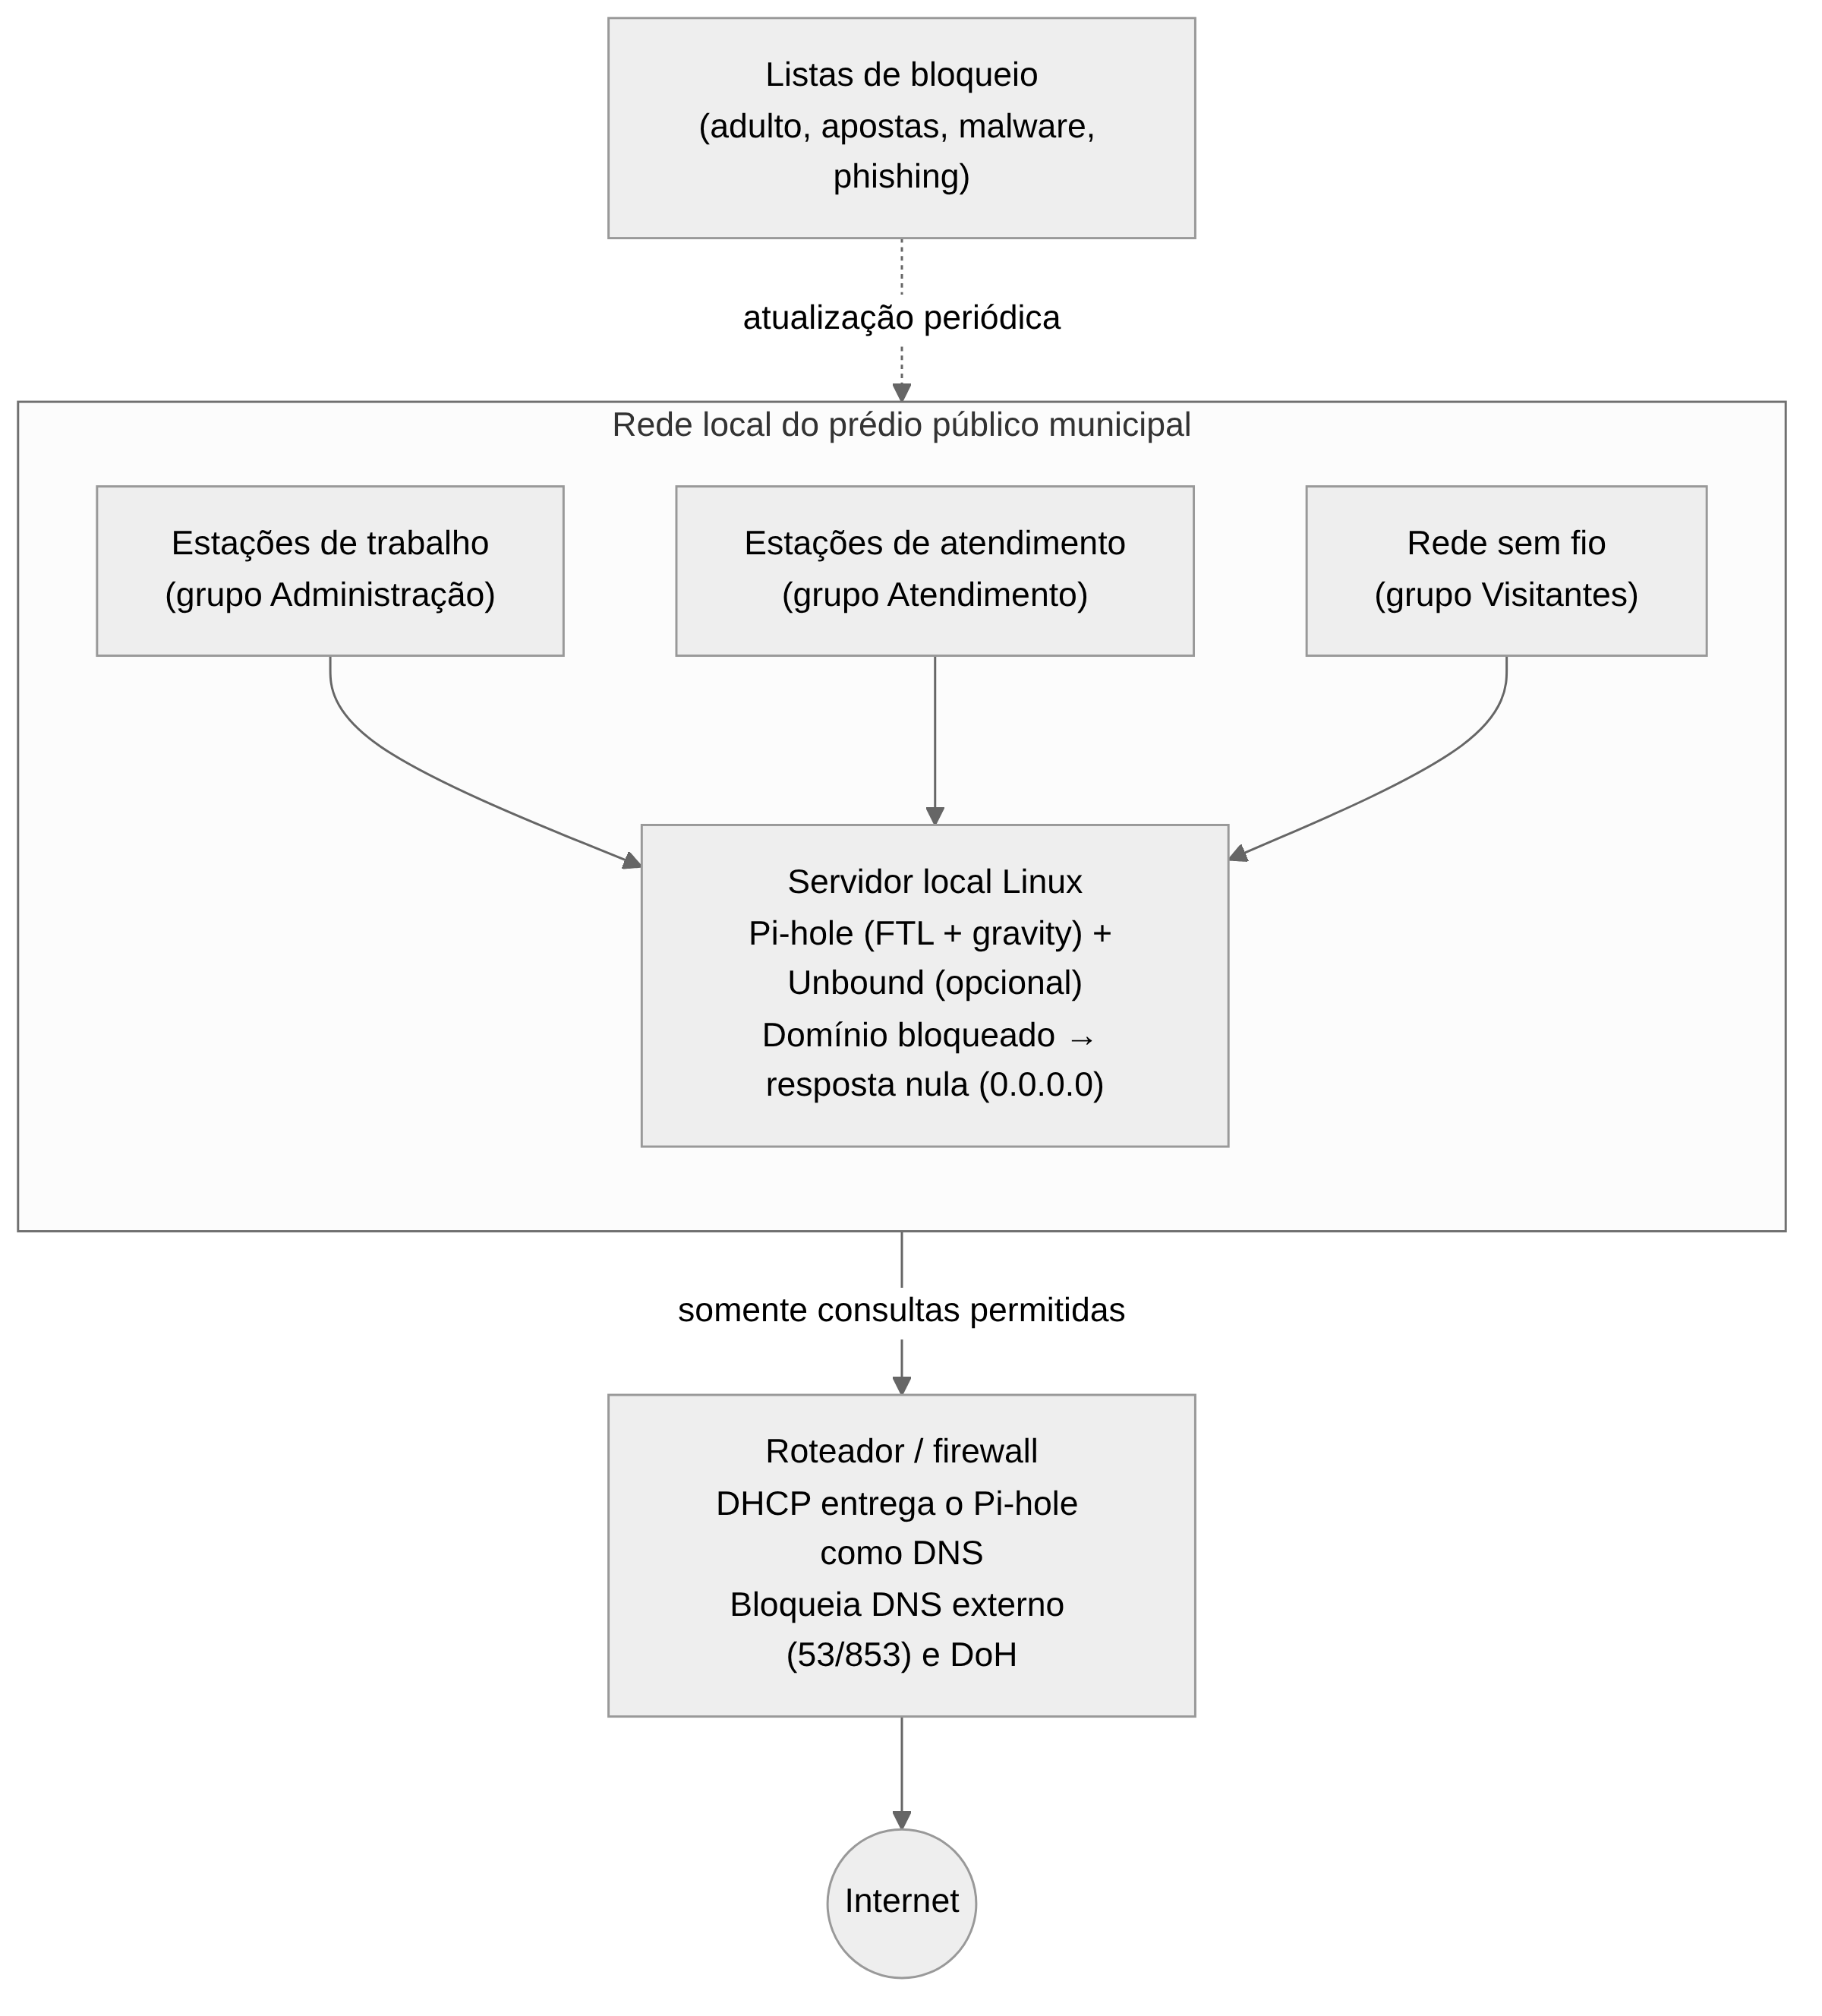
\includegraphics[height=0.62\textheight,keepaspectratio]{arquitetura.png}\end{center}\end{spacing}
\begin{spacing}{1}\noindent{\fontsize{10}{12}\selectfont Fonte: Elaborado pelo autor (2026).}\par\vspace{10pt}\end{spacing}
A solução é composta por quatro elementos:

{\leftskip=1.25cm\noindent\hangindent=0.6cm a)~ servidor local: computador ou máquina virtual com Linux, endereço IP fixo, Pi-hole e, opcionalmente, Unbound como resolvedor recursivo;\par}
{\leftskip=1.25cm\noindent\hangindent=0.6cm b)~ políticas de filtragem: listas de bloqueio por categoria, expressões regulares, lista de permissão para sistemas governamentais e grupos, por exemplo, "Administração", "Atendimento" e "Visitantes", com regras distintas;\par}
{\leftskip=1.25cm\noindent\hangindent=0.6cm c)~ medidas complementares de rede: DHCP do roteador apontando o Pi-hole como único DNS e regras de \textit{firewall} que bloqueiem DNS externo (portas 53 e 853) e domínios conhecidos de DoH;\par}
{\leftskip=1.25cm\noindent\hangindent=0.6cm d)~ gestão e governança: painel de acompanhamento, nível de privacidade definido, retenção limitada de registros, \textit{backup} periódico das configurações e minuta de política de uso aceitável da internet, a ser apresentada à gestão municipal.\par}
Além do controle de conteúdo, a solução agrega outras funcionalidades de segurança e de gestão: bloqueio de domínios de \textit{malware} e \textit{phishing}, bloqueio de anúncios e rastreadores, com redução do consumo de banda, e geração de estatísticas de uso que apoiam a tomada de decisão. Como possível desdobramento, caso o cronograma permita, poderá ser desenvolvido um pequeno painel de relatórios gerenciais em PHP que consuma a API REST do Pi-hole e apresente indicadores agregados à gestão, sem expor dados individuais.

\subsection{Análise dos dados}
Os dados quantitativos serão organizados em planilhas e analisados por estatística descritiva, com cálculo de frequências, percentuais, médias e medianas, e apresentados em tabelas e gráficos. As respostas da entrevista serão examinadas por meio de análise de conteúdo, com categorização temática (BARDIN, 2016), de modo a identificar necessidades, restrições e expectativas do órgão em relação ao controle de acesso. A confrontação entre os resultados dos testes e as hipóteses permitirá confirmá-las ou refutá-las e responder à questão norteadora.

\subsection{Aspectos éticos}
A pesquisa será iniciada somente após a obtenção de termo de anuência da instituição. A entrevista com o responsável técnico tratará exclusivamente da infraestrutura e dos procedimentos do órgão, e o entrevistado assinará termo de consentimento livre e esclarecido. Os registros do Pi-hole utilizados na análise serão agregados e anonimizados, com o uso dos níveis de privacidade da própria ferramenta, sem identificação de servidores, em conformidade com a LGPD (BRASIL, 2018b). A necessidade de submissão ao Comitê de Ética em Pesquisa será verificada com o orientador, à luz da Resolução nº 510/2016 do Conselho Nacional de Saúde (BRASIL, 2016).

\clearpage
\section{CRONOGRAMA}
O Quadro 3 apresenta a distribuição das atividades ao longo do período de execução, de outubro de 2026 a março de 2027, que poderá ser ajustada ao calendário acadêmico do curso e à autorização da instituição para a realização do piloto.

\begin{spacing}{1}\noindent\textbf{Quadro 3 --} Cronograma de execução da pesquisa\par\vspace{3pt}\nopagebreak
\noindent{\fontsize{10}{12}\selectfont\renewcommand{\arraystretch}{1.2}
\begin{tabular}{|p{0.40\textwidth}|>{\centering\arraybackslash}p{0.07\textwidth}|>{\centering\arraybackslash}p{0.07\textwidth}|>{\centering\arraybackslash}p{0.07\textwidth}|>{\centering\arraybackslash}p{0.07\textwidth}|>{\centering\arraybackslash}p{0.07\textwidth}|>{\centering\arraybackslash}p{0.07\textwidth}|}
\hline
\textbf{Atividades} & \textbf{Out.} & \textbf{Nov.} & \textbf{Dez.} & \textbf{Jan.} & \textbf{Fev.} & \textbf{Mar.} \\ \hline
Levantamento bibliográfico e documental & $\bullet$ & $\bullet$ & $\bullet$ &  &  &  \\ \hline
Elaboração e entrega do projeto de pesquisa & $\bullet$ & $\bullet$ &  &  &  &  \\ \hline
Orientações com o orientador & $\bullet$ & $\bullet$ & $\bullet$ & $\bullet$ & $\bullet$ & $\bullet$ \\ \hline
Obtenção do termo de anuência e diagnóstico da rede &  &  & $\bullet$ &  &  &  \\ \hline
Implantação do Pi-hole em ambiente de homologação &  &  & $\bullet$ & $\bullet$ &  &  \\ \hline
Testes de bloqueio, desempenho e contorno &  &  &  & $\bullet$ &  &  \\ \hline
Piloto em um setor (se autorizado) &  &  &  & $\bullet$ & $\bullet$ &  \\ \hline
Análise dos dados &  &  &  &  & $\bullet$ &  \\ \hline
Elaboração da proposta tecnológica e do texto final &  &  &  &  & $\bullet$ & $\bullet$ \\ \hline
Apresentação à banca examinadora &  &  &  &  &  & $\bullet$ \\ \hline
\end{tabular}}\par\end{spacing}
\begin{spacing}{1}\noindent{\fontsize{10}{12}\selectfont Fonte: Elaborado pelo autor (2026).}\par\vspace{10pt}\end{spacing}
\clearpage
\begin{center}\textbf{REFERÊNCIAS}\end{center}
\addcontentsline{toc}{section}{REFERÊNCIAS}
\vspace{6pt}
\begin{spacing}{1}\raggedright\noindent ARRUDA, Guilherme. Ciberataques no Brasil em 2025: prejuízos e falhas expostas. \textbf{WeLiveSecurity}, [\textit{s. l.}], 25 ago. 2025. Disponível em: \url{https://www.welivesecurity.com/pt/seguranca-digital/ciberataques-no-brasil-em-2025-prejuizos-e-falhas-expostas/}. Acesso em: 26 out. 2026.\par\vspace{12pt}\end{spacing}
\begin{spacing}{1}\raggedright\noindent ASSOCIAÇÃO BRASILEIRA DE NORMAS TÉCNICAS. \textbf{ABNT NBR ISO/IEC 27001}: segurança da informação, segurança cibernética e proteção à privacidade: sistemas de gestão da segurança da informação: requisitos. Rio de Janeiro: ABNT, 2022a.\par\vspace{12pt}\end{spacing}
\begin{spacing}{1}\raggedright\noindent ASSOCIAÇÃO BRASILEIRA DE NORMAS TÉCNICAS. \textbf{ABNT NBR ISO/IEC 27002}: segurança da informação, segurança cibernética e proteção à privacidade: controles de segurança da informação. Rio de Janeiro: ABNT, 2022b.\par\vspace{12pt}\end{spacing}
\begin{spacing}{1}\raggedright\noindent BARDIN, Laurence. \textbf{Análise de conteúdo}. São Paulo: Edições 70, 2016.\par\vspace{12pt}\end{spacing}
\begin{spacing}{1}\raggedright\noindent BLACK, Steven. \textbf{Hosts}: consolidating and extending hosts files from several well-curated sources. [\textit{S. l.}]: GitHub, 2025. Disponível em: \url{https://github.com/StevenBlack/hosts}. Acesso em: 26 out. 2026.\par\vspace{12pt}\end{spacing}
\begin{spacing}{1}\raggedright\noindent BRASIL. Lei nº 8.069, de 13 de julho de 1990. Dispõe sobre o Estatuto da Criança e do Adolescente e dá outras providências. \textbf{Diário Oficial da União}: seção 1, Brasília, DF, 16 jul. 1990. Disponível em: \url{https://www.planalto.gov.br/ccivil_03/leis/l8069.htm}. Acesso em: 26 out. 2026.\par\vspace{12pt}\end{spacing}
\begin{spacing}{1}\raggedright\noindent BRASIL. Lei nº 12.737, de 30 de novembro de 2012. Dispõe sobre a tipificação criminal de delitos informáticos; altera o Decreto-Lei nº 2.848, de 7 de dezembro de 1940 - Código Penal; e dá outras providências. \textbf{Diário Oficial da União}: seção 1, Brasília, DF, 3 dez. 2012. Disponível em: \url{https://www.planalto.gov.br/ccivil_03/_ato2011-2014/2012/lei/l12737.htm}. Acesso em: 26 out. 2026.\par\vspace{12pt}\end{spacing}
\begin{spacing}{1}\raggedright\noindent BRASIL. Lei nº 12.965, de 23 de abril de 2014. Estabelece princípios, garantias, direitos e deveres para o uso da Internet no Brasil. \textbf{Diário Oficial da União}: seção 1, Brasília, DF, 24 abr. 2014. Disponível em: \url{https://www.planalto.gov.br/ccivil_03/_ato2011-2014/2014/lei/l12965.htm}. Acesso em: 26 out. 2026.\par\vspace{12pt}\end{spacing}
\begin{spacing}{1}\raggedright\noindent BRASIL. Conselho Nacional de Saúde. Resolução nº 510, de 7 de abril de 2016. Dispõe sobre as normas aplicáveis a pesquisas em Ciências Humanas e Sociais. \textbf{Diário Oficial da União}: seção 1, Brasília, DF, 24 maio 2016. Disponível em: \url{https://conselho.saude.gov.br/resolucoes/2016/Reso510.pdf}. Acesso em: 26 out. 2026.\par\vspace{12pt}\end{spacing}
\begin{spacing}{1}\raggedright\noindent BRASIL. Decreto nº 9.637, de 26 de dezembro de 2018. Institui a Política Nacional de Segurança da Informação, dispõe sobre a governança da segurança da informação, e altera o Decreto nº 2.295, de 4 de agosto de 1997. \textbf{Diário Oficial da União}: seção 1, Brasília, DF, 27 dez. 2018a. Disponível em: \url{https://www.planalto.gov.br/ccivil_03/_ato2015-2018/2018/decreto/d9637.htm}. Acesso em: 26 out. 2026.\par\vspace{12pt}\end{spacing}
\begin{spacing}{1}\raggedright\noindent BRASIL. Lei nº 13.709, de 14 de agosto de 2018. Lei Geral de Proteção de Dados Pessoais (LGPD). \textbf{Diário Oficial da União}: seção 1, Brasília, DF, 15 ago. 2018b. Disponível em: \url{https://www.planalto.gov.br/ccivil_03/_ato2015-2018/2018/lei/l13709.htm}. Acesso em: 26 out. 2026.\par\vspace{12pt}\end{spacing}
\begin{spacing}{1}\raggedright\noindent BRASIL. Decreto nº 11.856, de 26 de dezembro de 2023. Institui a Política Nacional de Cibersegurança e o Comitê Nacional de Cibersegurança. \textbf{Diário Oficial da União}: seção 1, Brasília, DF, 27 dez. 2023. Disponível em: \url{https://www.planalto.gov.br/ccivil_03/_ato2023-2026/2023/decreto/d11856.htm}. Acesso em: 26 out. 2026.\par\vspace{12pt}\end{spacing}
\begin{spacing}{1}\raggedright\noindent BRASIL. Ministério da Gestão e da Inovação em Serviços Públicos. Secretaria de Governo Digital. \textbf{Guia do framework de privacidade e segurança da informação}. Versão 1.1.3. Brasília, DF: SGD, 2024. Disponível em: \url{https://www.gov.br/governodigital/pt-br/privacidade-e-seguranca/ppsi/guia_framework_psi.pdf}. Acesso em: 26 out. 2026.\par\vspace{12pt}\end{spacing}
\begin{spacing}{1}\raggedright\noindent CENTER FOR INTERNET SECURITY. \textbf{CIS Critical Security Controls}: version 8.1. East Greenbush, NY: CIS, 2024. Disponível em: \url{https://www.cisecurity.org/insights/white-papers/cis-critical-security-controls-v8-1}. Acesso em: 26 out. 2026.\par\vspace{12pt}\end{spacing}
\begin{spacing}{1}\raggedright\noindent CENTRO REGIONAL DE ESTUDOS PARA O DESENVOLVIMENTO DA SOCIEDADE DA INFORMAÇÃO. \textbf{TIC Governo Eletrônico 2023}: pesquisa sobre o uso das tecnologias de informação e comunicação no setor público brasileiro: resumo executivo. São Paulo: Comitê Gestor da Internet no Brasil, 2024. Disponível em: \url{https://cetic.br/media/docs/publicacoes/2/20240826104230/resumo_executivo_tic_governo_eletronico_2023.pdf}. Acesso em: 26 out. 2026.\par\vspace{12pt}\end{spacing}
\begin{spacing}{1}\raggedright\noindent CYBERSECURITY AND INFRASTRUCTURE SECURITY AGENCY. \textbf{Encrypted DNS implementation guidance}. Version 1.0. Washington, DC: CISA, 2024. Disponível em: \url{https://www.cisa.gov/sites/default/files/2024-05/Encrypted%20DNS%20Implementation%20Guidance_508c.pdf}. Acesso em: 26 out. 2026.\par\vspace{12pt}\end{spacing}
\begin{spacing}{1}\raggedright\noindent DRESCH, Aline; LACERDA, Daniel Pacheco; ANTUNES JÚNIOR, José Antonio Valle. \textbf{Design science research}: método de pesquisa para avanço da ciência e tecnologia. Porto Alegre: Bookman, 2015.\par\vspace{12pt}\end{spacing}
\begin{spacing}{1}\raggedright\noindent ELAVARASI, R. \textit{et al}. Enhancing network security and content control in academic environments using Pi-hole. \textbf{Journal of Applied Data Sciences}, [\textit{s. l.}], v. 7, n. 3, p. 2504-2515, set. 2026. DOI: \url{https://doi.org/10.47738/jads.v7i3.1472}.\par\vspace{12pt}\end{spacing}
\begin{spacing}{1}\raggedright\noindent GIL, Antonio Carlos. \textbf{Como elaborar projetos de pesquisa}. 7. ed. Barueri, SP: Atlas, 2022.\par\vspace{12pt}\end{spacing}
\begin{spacing}{1}\raggedright\noindent HEVNER, Alan R. \textit{et al}. Design science in information systems research. \textbf{MIS Quarterly}, Minneapolis, v. 28, n. 1, p. 75-105, 2004.\par\vspace{12pt}\end{spacing}
\begin{spacing}{1}\raggedright\noindent HOFFMAN, Paul; MCMANUS, Patrick. \textbf{RFC 8484}: DNS queries over HTTPS (DoH). [\textit{S. l.}]: IETF, 2018. DOI: \url{https://doi.org/10.17487/RFC8484}.\par\vspace{12pt}\end{spacing}
\begin{spacing}{1}\raggedright\noindent HOUNSEL, Austin \textit{et al}. Comparing the effects of DNS, DoT, and DoH on web performance. \textit{In}: THE WEB CONFERENCE, 29., 2020, Taipei. \textbf{Proceedings} [...]. New York: ACM, 2020. DOI: \url{https://doi.org/10.1145/3366423.3380139}.\par\vspace{12pt}\end{spacing}
\begin{spacing}{1}\raggedright\noindent HU, Zi \textit{et al}. \textbf{RFC 7858}: specification for DNS over Transport Layer Security (TLS). [\textit{S. l.}]: IETF, 2016. DOI: \url{https://doi.org/10.17487/RFC7858}.\par\vspace{12pt}\end{spacing}
\begin{spacing}{1}\raggedright\noindent KHORMALI, Aminollah \textit{et al}. Domain name system security and privacy: a contemporary survey. \textbf{arXiv}, [\textit{s. l.}], 2020. Preprint arXiv:2006.15277. Disponível em: \url{https://arxiv.org/abs/2006.15277}. Acesso em: 26 out. 2026.\par\vspace{12pt}\end{spacing}
\begin{spacing}{1}\raggedright\noindent KÜHRER, Marc; ROSSOW, Christian; HOLZ, Thorsten. Paint it black: evaluating the effectiveness of malware blacklists. \textit{In}: INTERNATIONAL SYMPOSIUM ON RESEARCH IN ATTACKS, INTRUSIONS AND DEFENSES, 17., 2014, Gothenburg. \textbf{Proceedings} [...]. Cham: Springer, 2014. p. 1-21. DOI: \url{https://doi.org/10.1007/978-3-319-11379-1_1}.\par\vspace{12pt}\end{spacing}
\begin{spacing}{1}\raggedright\noindent KUROSE, James F.; ROSS, Keith W. \textbf{Redes de computadores e a Internet}: uma abordagem top-down. 8. ed. Porto Alegre: Bookman, 2021.\par\vspace{12pt}\end{spacing}
\begin{spacing}{1}\raggedright\noindent MARCONI, Marina de Andrade; LAKATOS, Eva Maria. \textbf{Fundamentos de metodologia científica}. 9. ed. São Paulo: Atlas, 2022.\par\vspace{12pt}\end{spacing}
\begin{spacing}{1}\raggedright\noindent MOCKAPETRIS, Paul. \textbf{RFC 1034}: domain names: concepts and facilities. [\textit{S. l.}]: IETF, 1987a. DOI: \url{https://doi.org/10.17487/RFC1034}.\par\vspace{12pt}\end{spacing}
\begin{spacing}{1}\raggedright\noindent MOCKAPETRIS, Paul. \textbf{RFC 1035}: domain names: implementation and specification. [\textit{S. l.}]: IETF, 1987b. DOI: \url{https://doi.org/10.17487/RFC1035}.\par\vspace{12pt}\end{spacing}
\begin{spacing}{1}\raggedright\noindent NATIONAL SECURITY AGENCY; CYBERSECURITY AND INFRASTRUCTURE SECURITY AGENCY. \textbf{Selecting a protective DNS service}. Fort Meade, MD: NSA, 2021. Disponível em: \url{https://www.nsa.gov/Press-Room/News-Highlights/Article/Article/2523771/nsa-and-cisa-release-cybersecurity-information-on-protective-dns/}. Acesso em: 26 out. 2026.\par\vspace{12pt}\end{spacing}
\begin{spacing}{1}\raggedright\noindent NLNET LABS. \textbf{Unbound documentation}. Amsterdam: NLnet Labs, 2025. Disponível em: \url{https://unbound.docs.nlnetlabs.nl/}. Acesso em: 26 out. 2026.\par\vspace{12pt}\end{spacing}
\begin{spacing}{1}\raggedright\noindent PI-HOLE. \textbf{Pi-hole documentation}. [\textit{S. l.}]: Pi-hole, 2025a. Disponível em: \url{https://docs.pi-hole.net/}. Acesso em: 26 out. 2026.\par\vspace{12pt}\end{spacing}
\begin{spacing}{1}\raggedright\noindent PI-HOLE. \textbf{Introducing Pi-hole v6}. [\textit{S. l.}]: Pi-hole, 18 fev. 2025b. Disponível em: \url{https://pi-hole.net/blog/2025/02/18/introducing-pi-hole-v6/}. Acesso em: 26 out. 2026.\par\vspace{12pt}\end{spacing}
\begin{spacing}{1}\raggedright\noindent ROSE, Scott; LIU, Cricket; GIBSON, Ross. \textbf{Secure Domain Name System (DNS) deployment guide}. Gaithersburg, MD: NIST, 2026. (NIST Special Publication 800-81r3). DOI: \url{https://doi.org/10.6028/NIST.SP.800-81r3}.\par\vspace{12pt}\end{spacing}
\begin{spacing}{1}\raggedright\noindent STALLINGS, William; BROWN, Lawrie. \textbf{Segurança de computadores}: princípios e práticas. 2. ed. Rio de Janeiro: Elsevier, 2014.\par\vspace{12pt}\end{spacing}
\begin{spacing}{1}\raggedright\noindent TANENBAUM, Andrew S.; FEAMSTER, Nick; WETHERALL, David J. \textbf{Redes de computadores}. 6. ed. Porto Alegre: Bookman, 2021.\par\vspace{12pt}\end{spacing}
\begin{spacing}{1}\raggedright\noindent UNIVERSITÉ TOULOUSE CAPITOLE. \textbf{Blacklists UT1}. Toulouse: Université Toulouse Capitole, 2025. Disponível em: \url{https://dsi.ut-capitole.fr/blacklists/}. Acesso em: 26 out. 2026.\par\vspace{12pt}\end{spacing}
\begin{spacing}{1}\raggedright\noindent WAZLAWICK, Raul Sidnei. \textbf{Metodologia de pesquisa para ciência da computação}. 2. ed. Rio de Janeiro: Elsevier, 2014.\par\vspace{12pt}\end{spacing}
\clearpage
\begin{center}\textbf{APÊNDICE A – ROTEIRO DE ENTREVISTA SEMIESTRUTURADA COM O RESPONSÁVEL TÉCNICO PELA REDE}\end{center}
\addcontentsline{toc}{section}{APÊNDICE A -- ROTEIRO DE ENTREVISTA SEMIESTRUTURADA COM O RESPONSÁVEL TÉCNICO PELA REDE}
\vspace{6pt}
{\leftskip=1.25cm\noindent\hangindent=0.6cm a)~ Qual é sua função e há quanto tempo é responsável pela rede deste prédio?\par}
{\leftskip=1.25cm\noindent\hangindent=0.6cm b)~ Quantos computadores, dispositivos e usuários utilizam a rede atualmente? Há rede sem fio para visitantes?\par}
{\leftskip=1.25cm\noindent\hangindent=0.6cm c)~ Qual equipamento faz a função de roteador, \textit{firewall} e servidor DHCP? Qual servidor DNS é distribuído hoje aos computadores?\par}
{\leftskip=1.25cm\noindent\hangindent=0.6cm d)~ Existe alguma política formal de uso da internet ou de segurança da informação no órgão?\par}
{\leftskip=1.25cm\noindent\hangindent=0.6cm e)~ Já ocorreram incidentes de segurança, como vírus, \textit{ransomware}, \textit{phishing} ou sequestro de contas? Como foram tratados?\par}
{\leftskip=1.25cm\noindent\hangindent=0.6cm f)~ Há registros ou relatos de acesso a conteúdo indevido a partir da rede? Que tipo de conteúdo preocupa mais a gestão?\par}
{\leftskip=1.25cm\noindent\hangindent=0.6cm g)~ Existe algum mecanismo atual de bloqueio ou de monitoramento de navegação? Qual?\par}
{\leftskip=1.25cm\noindent\hangindent=0.6cm h)~ Quais sistemas e sítios eletrônicos são indispensáveis ao funcionamento do órgão e não podem ser bloqueados?\par}
{\leftskip=1.25cm\noindent\hangindent=0.6cm i)~ Quais restrições existem para a instalação de um servidor local, como disponibilidade de equipamento, energia, espaço e acesso administrativo ao roteador?\par}
{\leftskip=1.25cm\noindent\hangindent=0.6cm j)~ Que funcionalidades, além do bloqueio de conteúdo, seriam úteis para a gestão de TI do órgão?\par}
\clearpage
\begin{center}\textbf{APÊNDICE B – CHECKLIST DE DIAGNÓSTICO DA REDE}\end{center}
\addcontentsline{toc}{section}{APÊNDICE B -- CHECKLIST DE DIAGNÓSTICO DA REDE}
\vspace{6pt}
\begin{spacing}{1}\noindent\textbf{Quadro 4 --} Checklist de diagnóstico da infraestrutura de rede\par\vspace{3pt}\nopagebreak
\noindent{\fontsize{10}{12}\selectfont\renewcommand{\arraystretch}{1.2}
\begin{tabular}{|>{\raggedright\arraybackslash}p{0.427\textwidth}|>{\raggedright\arraybackslash}p{0.267\textwidth}|>{\raggedright\arraybackslash}p{0.267\textwidth}|}
\hline
\textbf{Item verificado} & \textbf{Situação encontrada} & \textbf{Observações} \\ \hline
Topologia da rede (cabeada/sem fio, \textit{switches}, segmentos) &  &  \\ \hline
Modelo do roteador/\textit{firewall} e possibilidade de criar regras de saída &  &  \\ \hline
Servidor DHCP utilizado e DNS distribuído atualmente &  &  \\ \hline
Número de estações e de dispositivos móveis conectados &  &  \\ \hline
Existência de rede separada para visitantes &  &  \\ \hline
Equipamento disponível para o servidor local (CPU, RAM, disco) ou hipervisor &  &  \\ \hline
Disponibilidade de \textit{nobreak} e local adequado para o servidor &  &  \\ \hline
Sistemas governamentais essenciais (lista de domínios a permitir) &  &  \\ \hline
Política de uso aceitável ou de segurança da informação vigente &  &  \\ \hline
Velocidade do \textit{link} de internet e provedor &  &  \\ \hline
\end{tabular}}\par\end{spacing}
\begin{spacing}{1}\noindent{\fontsize{10}{12}\selectfont Fonte: Elaborado pelo autor (2026).}\par\vspace{10pt}\end{spacing}
\end{document}
